\documentclass[tikz,border=12pt]{standalone}
\usepackage{tikz}
\usetikzlibrary{shapes.geometric,arrows.meta,positioning,fit,backgrounds,calc}

\renewcommand{\familydefault}{\sfdefault}
\definecolor{cborder}{HTML}{1E293B}
\definecolor{cbg}{HTML}{F8FAFC}
\definecolor{cbox}{HTML}{FFFFFF}
\definecolor{cblue}{HTML}{1E40AF}
\definecolor{cbluelight}{HTML}{EFF6FF}
\definecolor{cgray}{HTML}{64748B}
\definecolor{cgreen}{HTML}{059669}

\begin{document}
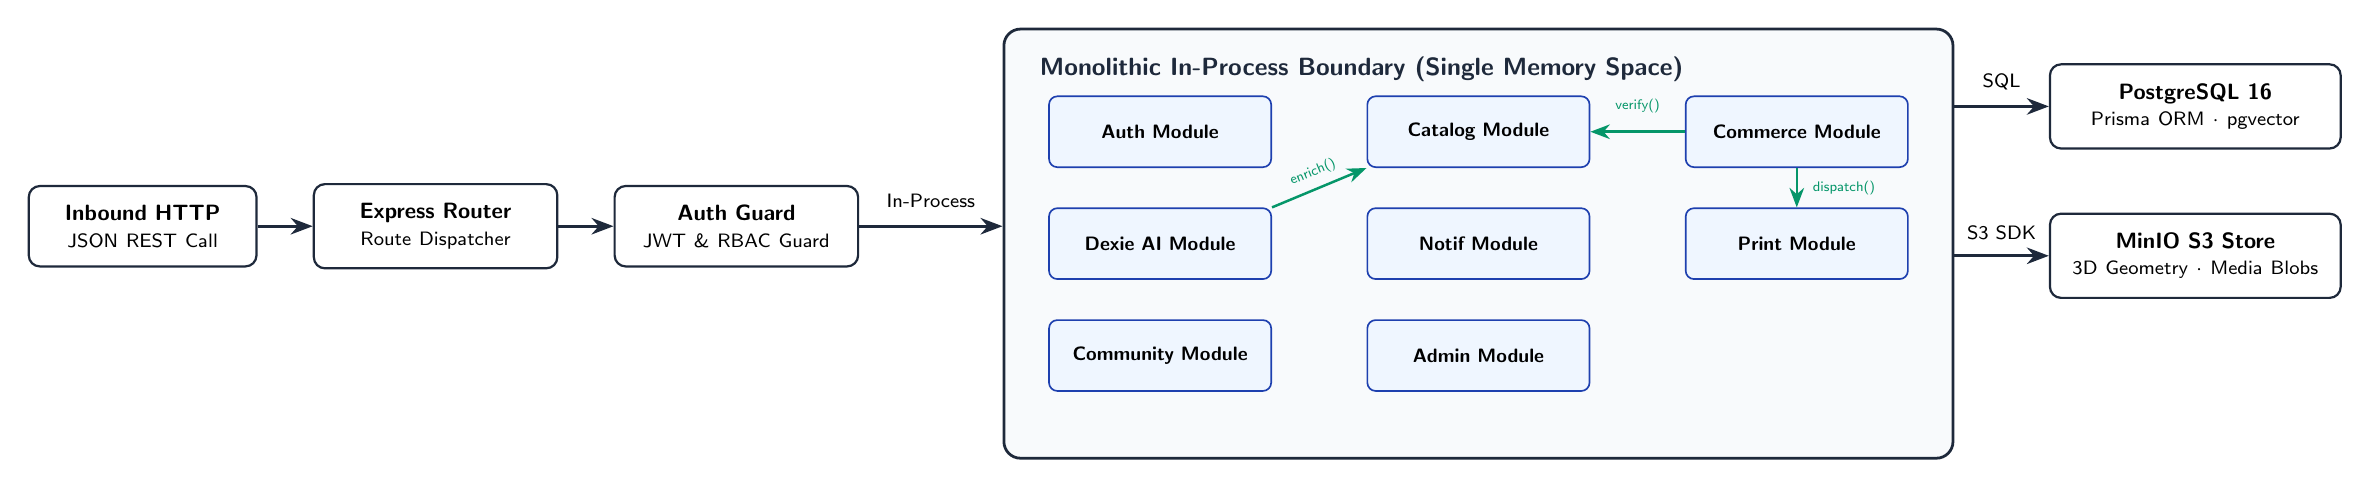
\begin{tikzpicture}[
    font=\small,
    >=Stealth,
    node distance=0.6cm and 0.8cm,
    block/.style={
        draw=cborder,
        fill=cbox,
        rounded corners=4pt,
        line width=0.8pt,
        align=center,
        inner sep=7pt,
        font=\footnotesize
    },
    mod/.style={
        draw=cblue,
        fill=cbluelight,
        rounded corners=3pt,
        line width=0.6pt,
        align=center,
        inner sep=6pt,
        font=\scriptsize,
        text width=2.4cm,
        minimum height=0.9cm
    },
    flow/.style={
        ->,
        line width=1.1pt,
        draw=cborder
    },
    localflow/.style={
        ->,
        line width=0.9pt,
        draw=cgreen
    }
]

    % Ingress pipeline on left
    \node[block, text width=2.4cm] (req) {
        \textbf{Inbound HTTP}\\
        \scriptsize JSON REST Call
    };

    \node[block, right=0.7cm of req, text width=2.6cm] (router) {
        \textbf{Express Router}\\
        \scriptsize Route Dispatcher
    };

    \node[block, right=0.7cm of router, text width=2.6cm] (guard) {
        \textbf{Auth Guard}\\
        \scriptsize JWT \& RBAC Guard
    };

    % Modules grid
    \node[mod, right=2.4cm of guard, yshift=1.2cm] (m_auth) {\textbf{Auth Module}};
    \node[mod, right=1.2cm of m_auth] (m_cat) {\textbf{Catalog Module}};
    \node[mod, right=1.2cm of m_cat] (m_com) {\textbf{Commerce Module}};

    \node[mod, below=0.5cm of m_auth] (m_dex) {\textbf{Dexie AI Module}};
    \node[mod, right=1.2cm of m_dex] (m_not) {\textbf{Notif Module}};
    \node[mod, right=1.2cm of m_not] (m_prt) {\textbf{Print Module}};

    \node[mod, below=0.5cm of m_dex] (m_soc) {\textbf{Community Module}};
    \node[mod, right=1.2cm of m_soc] (m_adm) {\textbf{Admin Module}};

    % Background container
    \begin{scope}[on background layer]
        \node[draw=cborder, fill=cbg, rounded corners=6pt, line width=1pt,
              fit=(m_auth) (m_cat) (m_com) (m_dex) (m_not) (m_prt) (m_soc) (m_adm),
              inner xsep=16pt, inner ysep=24pt] (mono_box) {};
    \end{scope}

    \node[anchor=north west, font=\bfseries\small, text=cborder] at (mono_box.north west) [xshift=10pt, yshift=-7pt] {
        Monolithic In-Process Boundary (Single Memory Space)
    };

    % Persistence nodes on right
    \node[block, right=1.2cm of mono_box.north east, yshift=-1.0cm, text width=3.2cm] (db_postgres) {
        \textbf{PostgreSQL 16}\\
        \scriptsize Prisma ORM $\cdot$ pgvector
    };

    \node[block, below=0.8cm of db_postgres, text width=3.2cm] (db_minio) {
        \textbf{MinIO S3 Store}\\
        \scriptsize 3D Geometry $\cdot$ Media Blobs
    };

    % Flow connections
    \draw[flow] (req) -- (router);
    \draw[flow] (router) -- (guard);
    \draw[flow] (guard) -- (guard -| mono_box.west) node[midway, above=3pt, font=\scriptsize] {In-Process};

    % Clean internal interactions
    \draw[localflow] (m_com.west) -- node[midway, above=3pt, font=\tiny, text=cgreen] {verify()} (m_cat.east);
    \draw[localflow] (m_com) -- (m_prt) node[midway, right=2pt, font=\tiny, text=cgreen] {dispatch()};
    \draw[localflow] (m_dex.north east) -- (m_cat.south west) node[midway, above=2pt, font=\tiny, text=cgreen, sloped, fill=cbg, inner sep=1pt] {enrich()};

    % Persistence flows
    \draw[flow] (mono_box.east |- db_postgres.west) -- (db_postgres.west)
        node[midway, above=2pt, font=\scriptsize] {SQL};
    \draw[flow] (mono_box.east |- db_minio.west) -- (db_minio.west)
        node[midway, above=2pt, font=\scriptsize] {S3 SDK};

\end{tikzpicture}
\end{document}
